\chapterimage{images/kotlin/kotlinprogramminglanguage.png}

\chapter{Hello Kotlin}
In this chapter we will cover some of the fundamentals of the basic Kotlin language. It is not meant to be an exhaustive overview and you will find none or very little code examples. The examples used can be found in the references spread around this chapter. 

\section{Kotlin vs. Java}

Kotlin was created with Java developers in mind, and with IntelliJ as its main development
IDE. There are several resources on why Kotlin has more advantages then Java. Maybe it is a good idea to have a look in the Kotlin documentation and see what they are telling. 

Go to this link: \url{https://kotlinlang.org/docs/reference/comparison-to-java.html}

The most important differences for this lesson are:

\begin{enumerate}
	\item Kotlin is null safe, which means that we deal with possible null
	situations in compile time, to prevent execution time exceptions. We need to
	explicitly specify that an object can be null, and then check its nullity before
	using it.
	\item As many other modern languages, it uses many
	concepts from functional programming, such as lambda expressions, to solve
	some problems in a much easier way. This was not possible in the Java-version of Android (at least not without the necessary extra libraries)
	\item It makes use of extension functions: This means we can extend any class
	with new features even if we don’t have access to the source code
\end{enumerate}

If you need a refresher regarding the advanced java concepts, we provide a small list explaining them (not in detail).

\begin{description}
	\item[Raw Type] Raw types refer to using a generic type without specifying a type parameter. For example, \texttt{List} is a raw type, while \texttt{List<String>} is a parameterized type. When generics were introduced in \gls{jdk} 1.5, raw types were retained only to maintain backwards compatibility with older versions of Java.
	\item[Checked Exception]: are the exceptions that are checked at compile time in java. If some code within a method throws a checked exception, then the method must either handle the exception or it must specify the exception using throws keyword.
	\item[Unchecked Exception] Unchecked are the exceptions that are not checked at compiled time.
	\item[Lambda expression] Provide a clear and concise way to represent one method interface using an expression. For a good introduction see \url{https://docs.oracle.com/javase/tutorial/java/javaOO/lambdaexpressions.html}
\end{description}

\section{Executing Kotling without Android}

You can use \url{try.kotlinlang.org} to test Kotling and some other simple examples without the need of
a real project. You could also use the \gls{repl} that comes bundled with the Kotlin plugin. You will
find it in Tools $\rightarrow$ Kotlin $\rightarrow$ Kotlin REPL..

\section{Classes}
The full description of classes can be found in this link \url{https://kotlinlang.org/docs/reference/classes.html}. This section only contains some pointers which you should not forget when programming. 

\subsection{Inheritance}
By default, a class always extends from Any (similar to Java Object), but we can
extend any other classes. Note however: Any is not  equals to thge java.lang.Object; in particular, it does not have any members other than equals(), hashCode() and toString() .Classes are closed by default (final), so we can only extend
a class if it’s explicitly declared as open or abstract.

\section{Functions}
Functions in Kotlin always return a value. So if you don’t specify a return value, it will return Unit.
Unit is similar to void in Java, though this is in fact an object. You can, of course,
specify any type as a return value.

Note that semicolons are not  necessary
and it’s a good practice to avoid them (the IDE will warn you).

You can use template expressions directly in your strings y prefixing with \$. This will make
it easy to write complex strings based on static and variable parts. 

\section{Exercises }
In this series of exercises we are going to cover the \gls{solid} design pattern and we will illustrate them with Kotlin code. Although the focus of these exercises is not de theory about these principles, we expect of course that you wil apply these principles in the nex chapters. 

If for some reason the authors  have forgotten to apply them in the examples, do not hesitate to  harass and try to disconcert us with with questions, challenges or gibes regarding these exercises. 


\subsection{\gls{solid} code}
S.O.L.I.D is an acronym for the first five object-oriented design \gls{ood} principles by Robert C. Martin.

These principles, when combined together, make it easy for a programmer to develop software that are easy to maintain and extend. They also make it easy for developers to easily refactor code and are also a part of the agile or adaptive software development.

We will list these principles in short:

\begin{description}
	\item[S] Single responsability principle
	\item[O] Open-closed principle
	\item[L] Liskov substitution principle
	\item[I] Interface segregation principle
	\item[D] Dependency Inversion Principle
\end{description}

The following subsection describes the principles in more detail. The figures have been retrieved from \cite{Devilla2009}.

\subsubsection{Single responsability principle }
\begin{framed}
The \gls{srp} states that a class should have one and only one reason to change, meaning that a class should have only one job.	
\end{framed}

\begin{figure}
	\centering
	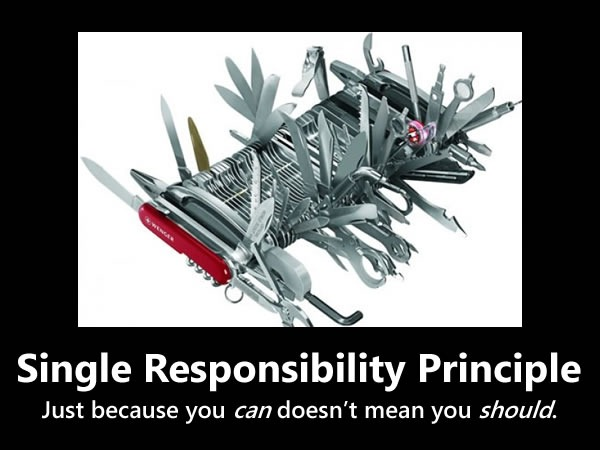
\includegraphics[width=0.8\textwidth]{images/kotlin/SRP.jpg}
	\caption{The “S” in \gls{solid} is for Single Responsibility Principle, which states that every object should have a single responsibility and that all of its services should be aligned with that responsibility. “Responsibility” is defined as “a reason to change”}
	\label{fir:SRP}
\end{figure}
As an example, consider an application that compiles and prints a book. Such an object can be changed for two reasons: \begin{inparaenum}[(i)]
	\item the content of the report can change and
	\item the format of the report can change.
\end{inparaenum}
 These two things change for very different causes; one substantive, and one cosmetic. The single responsibility principle says that these two aspects of the problem are really two separate responsibilities, and should therefore be in separate classes or modules. It would be a bad design to couple two things that change for different reasons at different times.

\begin{exercise}
	Let's have a look at the code in listing \ref{code:KotlinSRPBook}. This is a simple implementation in Kotlin which could implement the requirements listed above, althought it does not abide the \gls{srp}. Write down for yourself why this is the case and make an implementation which does abide the \gls{srp}.
\end{exercise}

\lstinputlisting[language=Kotlin, caption={The Kotlin code describing a book. This source code does not abide the Single Responsability Principle.}, label=code:KotlinSRPBook]{srccode/kotlin/book.kt}

\subsubsection{Open-Closed Principle}

\begin{figure}
	\centering
	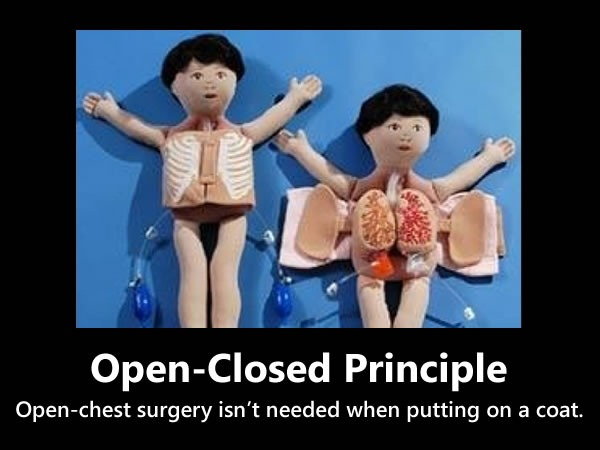
\includegraphics[width=0.8\textwidth]{images/kotlin/OCP.jpg}
	\caption{The “O” in \gls{solid} is for \gls{ocp}, which states that software entities such as classes, modules, functions and so on should be open for extension but closed for modification. The idea is that it’s often better to make changes to things like classes by adding to or building on top of them (using mechanisms like subclassing or polymorphism) rather than modifying their code.}
	\label{fir:OCP}
\end{figure}


\begin{framed}
	The \gls{ocp} states that software entities (classes, modules, functions, etc.) should be open for extension, but closed for modification, i.e.  such an entity can allow its behaviour to be extended without modifying its source code.
\end{framed}

The \gls{ocp} is tightly coupled with the Single \gls{srp}. If we design a class with SRP in mind, it is very likely that we also respect OCP or that little work is required to meet both, and vice versa. Think about the following example. 

Let’s say that we’ve got a Rectangle class with s a width and a height and we want to build an application that can calculate the total area of a collection of rectangles. See the rectangle code in \ref{code:KotlinOCPRectangle}.

\lstinputlisting[language=Kotlin, caption={The source code describing a rectangle.}, label=code:KotlinOCPRectangle]{srccode/kotlin/Rectangle.kt}

That’s not a problem for us. We learned in school that the area of a rectangle is it’s width multiplied with it’s height and we come up with the solution provided in TODO REF

\lstinputlisting[language=Kotlin, caption={The code to calculate the area of a rectangle.}, label=code:KotlinOCPArea]{srccode/kotlin/AreaCalculator.kt}


Now write down what the problem is with this solution. What, in this solution I need to calculate the area of a circle. What things do I need to adjust? 

\begin{exercise}
	Think about the things you have written and create the code which implements the \gls{srp} and the  \gls{ocp} correctly. 
\end{exercise}

\subsubsection{Liskov Substitution Principle}


\begin{framed}
	The \gls{lsp} states that functions that use pointers or references to base classes must be able to use objects of derived classes without knowing it.
\end{framed}
\begin{figure}
	\centering
	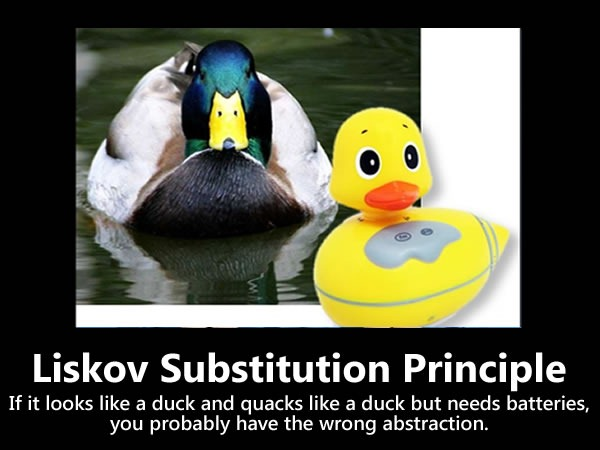
\includegraphics[width=0.8\textwidth]{images/kotlin/LSP.jpg}
	\caption{The “L” in \gls{solid} is for \gls{lsp} which states that subclases should be substitutable for the classes from which they were derived. For example, if MySubclass is a subclass of MyClass, you should be able to replace MyClass with MySubclass without bunging up the program.}
	\label{fir:LSP}
\end{figure}
A great example illustrating \gls{lsp}  was how sometimes something that sounds right in natural language doesn't quite work in code.

In mathematics, a Square is a Rectangle. Indeed it is a specialization of a rectangle. The "is a" makes you want to model this with inheritance. However if in code you made Square derive from Rectangle, then a Square should be usable anywhere you expect a Rectangle. This makes for some strange behavior which needs to override of functions which normally should not be overwritten. See the code in listing \ref{code:KotlinLSP}.

\lstinputlisting[language=Kotlin, caption={Implementation of a square by inheriting from Rectangle}, label=code:KotlinLSP]{srccode/kotlin/Square.kt}


Imagine you had SetWidth and SetHeight methods on your Rectangle base class; this seems perfectly logical. However if your Rectangle reference pointed to a Square, then SetWidth and SetHeight doesn't make sense because setting one would change the other to match it. In this case Square fails the Liskov Substitution Test with Rectangle and the abstraction of having Square inherit from Rectangle is a bad one.



\begin{exercise}
	Make an implementation of the Square and Rectangle which implements the \gls{srp},  \gls{ocp}  and the \gls{lsp} correctly. 
\end{exercise}